\documentclass[11pt]{article}
\usepackage[top=2cm,bottom=2cm,left=2.5cm,right= 2.5cm]{geometry}
%\geometry{landscape}                % Activate for for rotated page geometry
\usepackage[parfill]{parskip}    % Activate to begin paragraphs with an empty line rather than an indent
\usepackage{graphicx}
\usepackage{amssymb}
\usepackage{epstopdf}
\usepackage{amsmath}            
\usepackage{multirow}    
\usepackage{hyperref}
\usepackage{changepage}
\usepackage{lscape}
\usepackage{ulem}
\usepackage{multicol}
\usepackage[usenames,dvipsnames]{color}       
\usepackage{enumerate}
\newcommand{\urlwofont}[1]{\urlstyle{same}\url{#1}}
\newcommand{\degree}{\ensuremath{^\circ}}

\DeclareGraphicsRule{.tif}{png}{.png}{`convert #1 `dirname #1`/`basename #1 .tif`.png}

%\newcommand{\soln}[1]{\textcolor{MidnightBlue}{\textit{#1}}}	% delete #1 to get rid of solutions for handouts
\newcommand{\soln}[1]{ }

%\newcommand{\solnMult}[1]{\textbf{\textcolor{MidnightBlue}{\textit{#1}}}}	% uncomment for solutions
\newcommand{\solnMult}[1]{ #1 }	% uncomment for handouts

%\newcommand{\type}[1]{ \textbf{\textcolor{red}{(#1)}} }	% uncomment for handouts
\newcommand{\type}[1]{ }	% uncomment for handouts


\begin{document}

Dr. \c{C}etinkaya Rundel \hfill Sta 101 \\
$\:$ \\
{\LARGE \textbf{Final Review} } \\

\textcolor{red}{\textbf{(If you catch any errors in the solutions, let me know!)}}

%Final exam is on Thursday, May 3 between 9am - 12pm. Please note that there will be no make-up exams in this class.
%
%The exam is cumulative (covers everything we have learned) with an emphasis on the material since the second midterm.
%
%When studying for the exam you should review the homework questions you've had so far as well as any other questions from the book in the sections we've covered. I've included a sample of problems and included worked out solutions below. You shouldn't limit your studying to just these problems, but I thought these would be good to have the detailed answers for. Also note that detailed solutions for all past homework assignments are posted on the course webpage.

\begin{enumerate}

%

\item \type{EDA} A recent housing survey was conducted to determine the price of a typical home in Glendale, CA. Glendale is mostly middle-class, with one very expensive suburb. The mean price of a
house was roughly \$650,000. Which of the following statements is most likely to be true?
\begin{enumerate}
\item Most houses in Glendale cost more than \$650,000.
\item \solnMult{Most houses in Glendale cost less than \$650,000.}
\item There are about as many houses in Glendale that cost more than \$650,000 than less than this amount.
\item We need to know the standard deviation to answer this question
\end{enumerate}

%

\item \type{EDA} The table below shows some summary statistics of the distributions of resident tuition at public and private medical schools.

\begin{center}
\begin{tabular}{l | c | c | c | c | c}
			& Min	& Q1 	& Median	& Q3 	& Max \\
\hline
Private		& \$6,550 	& \$30,729	& \$33,850	& \$36,685	& \$41,360 \\
Public		& \$0 	& \$10,219	& \$16,168	& \$18,800	& \$27,886 \\
\end{tabular}
\end{center}


Determine which of the following statements is true about the spread for medical school
resident tuition.
\begin{enumerate}
\item The ranges of the two distributions are roughly equal indicating that the variability is the same for the two distributions.
\item \solnMult{There is more variation in tuitions for residents at public medical schools than at private medical schools since the interquartile range is higher for public schools.}
\item There is more variation in tuitions for residents at private medical schools than at public medical schools since there are outliers for private schools.
\item With these data, we cannot compare the variations of tuitions for residents at private and public medical schools.
\end{enumerate}

%

\item \type{EDA} The histograms below show the distributions of the duration of eruptions and waiting time between eruptions at the Old Faithful geyser in Yellowstone National Park, Wyoming, USA. 
\begin{center}
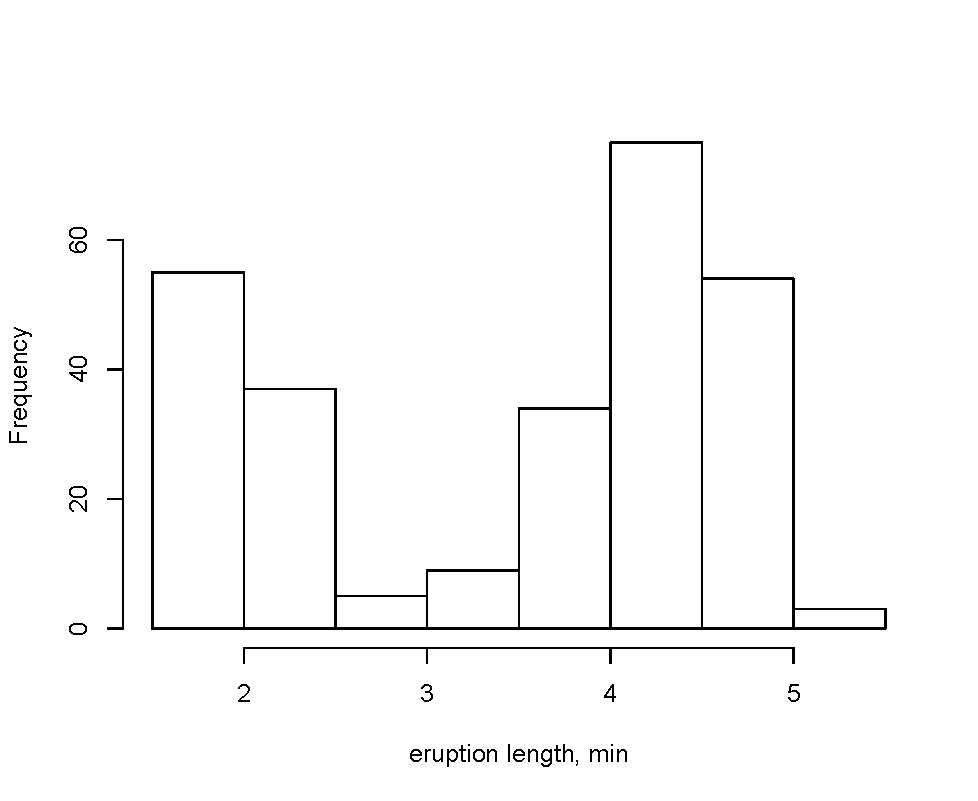
\includegraphics[width = 0.4\textwidth]{figures/erupt_length}
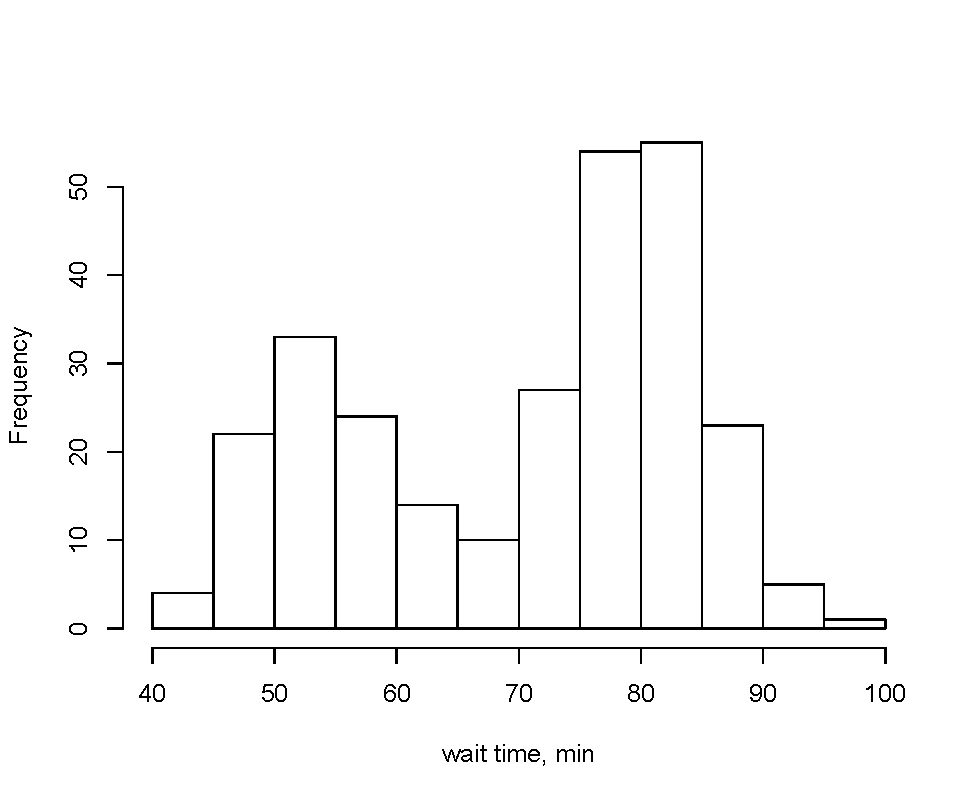
\includegraphics[width = 0.4\textwidth]{figures/wait_time}
\end{center}

\begin{enumerate}

\item Comment on the modality of the two variables.

\soln{Both distributions are bimodal. Eruption lengths are centered around 2 minutes and 4 minutes, and wait times are centered around 50 minutes and 80 minutes.}

\item Below is a scatterplot of the two variables. Describe the relationship and comment on how this scatterplot relates to the histograms.

\begin{center}
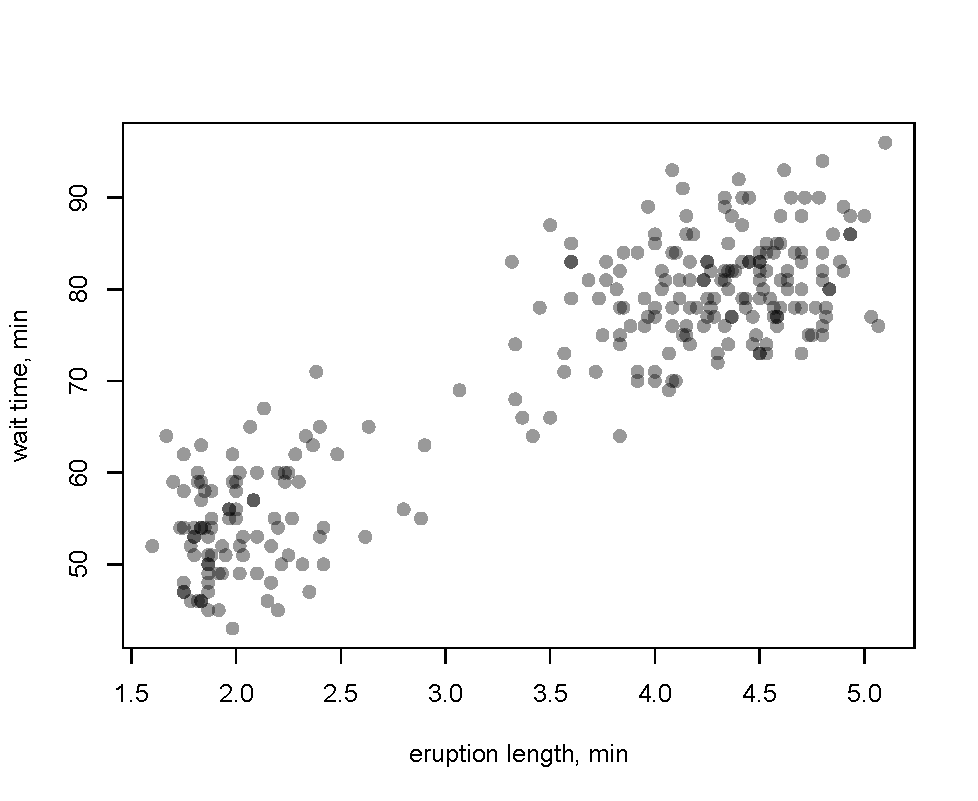
\includegraphics[width = 0.45\textwidth]{figures/faithful}
\end{center}

\soln{The relationship is positive, linear, and somewhat strong. However there isn't really constant variance. The points seem to be clustered around 2 and 4.5 minute equation lengths, same as in the histogram. It seems like there are two types of eruptions: short eruptions with short wait times in between, and longer eruptions with longer wait times in between.}

\end{enumerate}

%

\item \type{Probability - general \& binomial} It is known that 80\% of people like peanut butter, 89\% like jelly, and 78\% like both.
\begin{enumerate}
\item If we pick one person at random, what is the chance s/he likes peanut butter or jelly?

\soln{P(PB or J) = 0.80 + 0.89 - 0.78 = 0.91}

\item How many people like either peanut butter or jelly, but not both?

\soln{P(PB but not J) + P(J but not PB) = (0.80 - 0.78) + (0.89 - 0.78) = 0.13}

\item Suppose you pick out 8 people at random, what is the chance that exactly 1 of the 8 likes
peanut butter but not jelly?

\soln{P(PB but not J) = 0.80 - 0.78 = 0.02 \\
P(k = 1) = ${8 \choose 1} * 0.02^1 * 0.98^7 = 8 * 0.02^1 * 0.98^7 = 0.14$}

\item Are ``liking peanut butter" and ``liking jelly" disjoint outcomes?

\soln{No, there are people who like both.}

\item Are ``liking peanut butter" and ``liking jelly" independent outcomes?

\soln{If ``liking peanut butter" and ``liking jelly" were independent outcomes, we would expect P(PB and J) to be 0.80 * 0.89 = 0.712. Since the probability of the intersection (and) is different, the two events are not independent. (Note that there are other equally valid approaches to answering this question, for example one involving conditional probabilities.)}

\end{enumerate}

%

\pagebreak

\item \type{Probability - normal} The cholesterol levels for women aged 20 to 34 follow an approximately Normal distribution with mean 185 milligrams per deciliter (mg/dl) and standard deviation 39 mg/dl. About 18.5\% of women are known to have high cholesterol. What is the cutoff cholesterol level for for being considered as having high cholesterol?

\soln{The Z-score associated with the highest 18.5\% of the standard normal distribution is roughly 0.9.
\[Z = \frac{X - 185}{39} = 0.9 \rightarrow X = 0.9 * 39 + 185 = 220.1~mg/dl \]
}

%

%\item \type{Probability - geometric \& binomial} LeBron James has a free-throw percentage of 74\%. Assume the free-throw shots are independent; that is, success or failure on one does not affect the chance of success on another shot.\footnote{Adapted from \textit{Introductory Statistics} by Gould and Ryan.}
%
%\begin{enumerate}
%\item What is the probability that he makes his first free-throw in a game?
%
%\soln{P(makes first free-throw) = 0.74}
%
%\item What is the probability that he missed two free-throws but makes the third one?
%
%\soln{P(miss) = 1 - 0.74 = 0.26 \\
%P(makes third free-throw) = $0.26^2 * 0.74 = 0.05$}
%
%\item If he has 600 free-throws in an upcoming season, how many would you expect him to miss, give or take how many?
%
%\soln{$\mu = 600 * 0.74 = 444$ \\
%$\sigma = \sqrt{600 * 0.74 * 0.26} = 10.7443$\\
%You should expect him to hit about 444 free-throws, give or take about 10.74.
%}
%
%\end{enumerate}

%

\item \type{Probability - normal approx to binom} Suppose a university announced that it admitted 2,500 students for the following year's freshman class. However, the university has dorm room spots for only 1,786 freshman students. If there is a 70\% chance that an admitted student will decide to accept the offer and attend this university, what is the what is the approximate probability that the university will not have enough dormitory room spots for the freshman class?

\soln{Let $X$ be the number of students among the 2,000 who decide to attend this university. $X$ has a binomial distribution with number of trials $n = 2,500$ and $p = 0.70$.  The university will not have enough spots if $X \ge 1787$, and we use the normal approximation to the Binomial to calculate this probability. The mean and standard deviation of this distribution are
\[ \mu = np = 2500 * 0.7 = 1750 \qquad \sigma = \sqrt{np(1-p)} = \sqrt{2500 * 0.7 * 0.3} = 23 \]
\[ P(X > 1787)  = P \left( Z > \frac{1787 - 1750}{23} \right) = P(Z > 1.61) = 1 -  0.9463 = 0.0537 \]
}

%

%\item  \type{Probability - Bayes} A student who is traveling by train through Europe decides not to buy a ticket for the train. The train is traveling through both France and Germany and as such he may be asked to show his ticket to either the French or the German train guard. 
%The probability of being caught without a ticket by the German guard is 0.8, and the probability of getting caught by the French guard is 0.3. The probabilities of each are independent from one another.\footnote{Adapted from http://www.ibmaths.com/free/ws/statsprob/conditional\%20trees.pdf}
%
%\begin{enumerate}
%
%\item  Draw a tree diagram to represent the information in the paragraph above. 
%
%\soln{
%\begin{center}
%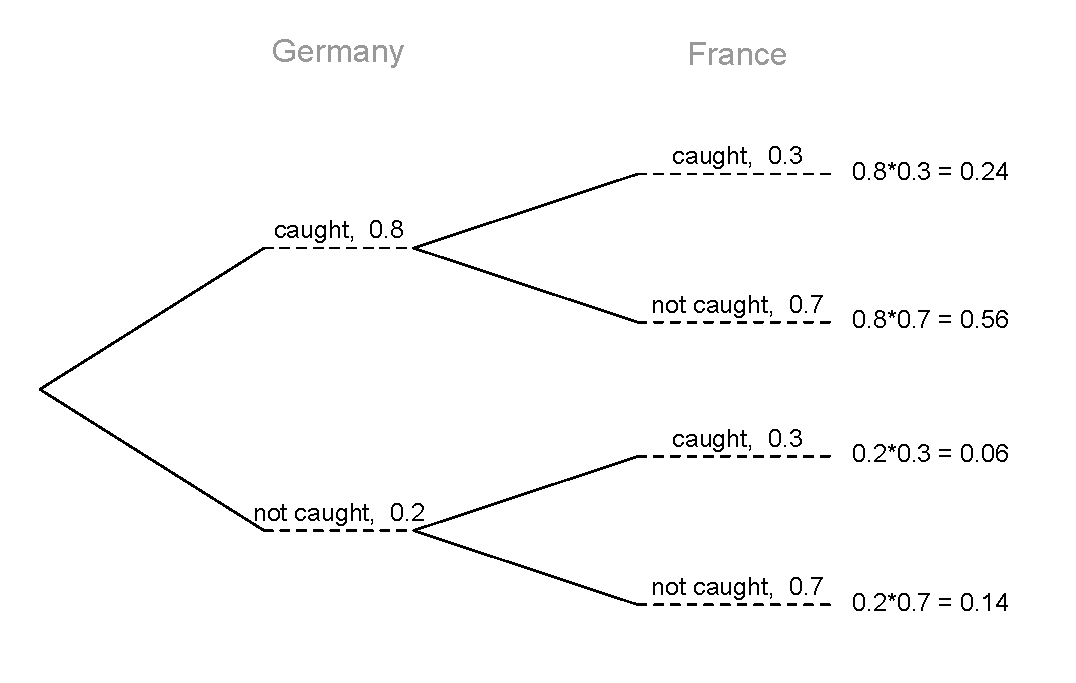
\includegraphics[width = 0.8\textwidth]{figures/tree}
%\end{center}
%}
%
%\item What is the probability of being caught by both of the guards?
%
%\soln{P(Germany AND France) = 0.24}
%
%\item What is the probability of being caught by either of the guards?
%
%\soln{Three approaches, all yield the same answer:
%P(Germany OR France) = 
%\begin{enumerate}[1.]
%\item P(Germany) + P(France) - P(Germany AND France) = 0.8 + 0.3 - 0.24 = 0.86
%\item P(Germany BUT not France) + P(France BUT not Germany) + P(Germany AND France) = 0.56 + 0.06 + 0.24 = 0.86
%\item 1 - P(NEITHER Germany NOR France) = 1 - 0.14 - 0.86
%\end{enumerate}
%}
%
%\item Given that the student has been caught by one of the guards only, find the probability that he was caught by,
%\begin{enumerate}
%\item the French guard,
%
%\soln{P(France $|$ caught by only one) = $\frac{ \text{P(France AND not Germany)} }{ \text{P(France AND not Germany) + P(Germany AND not France)} }$ \\
%= $\frac{0.06}{0.06 + 0.56} = 0.0967$
%}
%
%\item the German guard
%
%\soln{P(Germany $|$ caught by only one) = $\frac{ \text{P(Germany AND not France)} }{ \text{P(France AND not Germany) + P(Germany AND not France)} }$ \\
%= $\frac{0.56}{0.06 + 0.56} = 0.9032$
%}
%\end{enumerate}
%
%\end{enumerate}
%
%%
%
%\soln{
%\textit{Here is an alternative way of thinking about the problem:}
%\begin{center}
%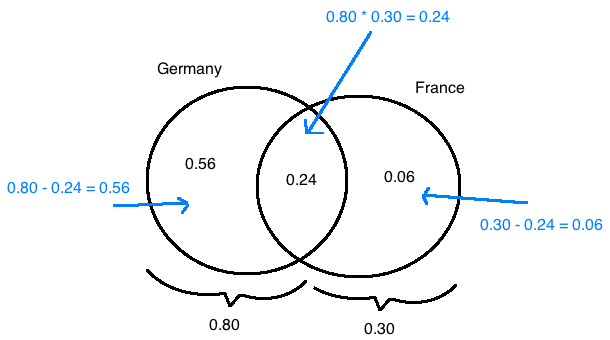
\includegraphics[width = 0.9\textwidth]{figures/train}
%\end{center}
%}

%

\item \type{Probability - Bayes} About 30\% of human twins are identical and the rest are fraternal. Identical twins are necessarily the same sex -- half are males and the other half are females. One-quarter of fraternal twins are both male, one-quarter both female, and one-half are mixes: one male, one female. You have just become a parent of twins and are told they are both girls. Given this information, what is the posterior probability that they are identical? \footnote{Adapted from \textit{Statistics: A Bayesian Perspective} by Berry.}

\soln{
\begin{align*}
P(identical~|~females) &= \frac{P(identical~and~females)}{P(females)} \\
&= \frac{0.15}{0.15+0.175} \\
&= 0.46
\end{align*}
\begin{center}
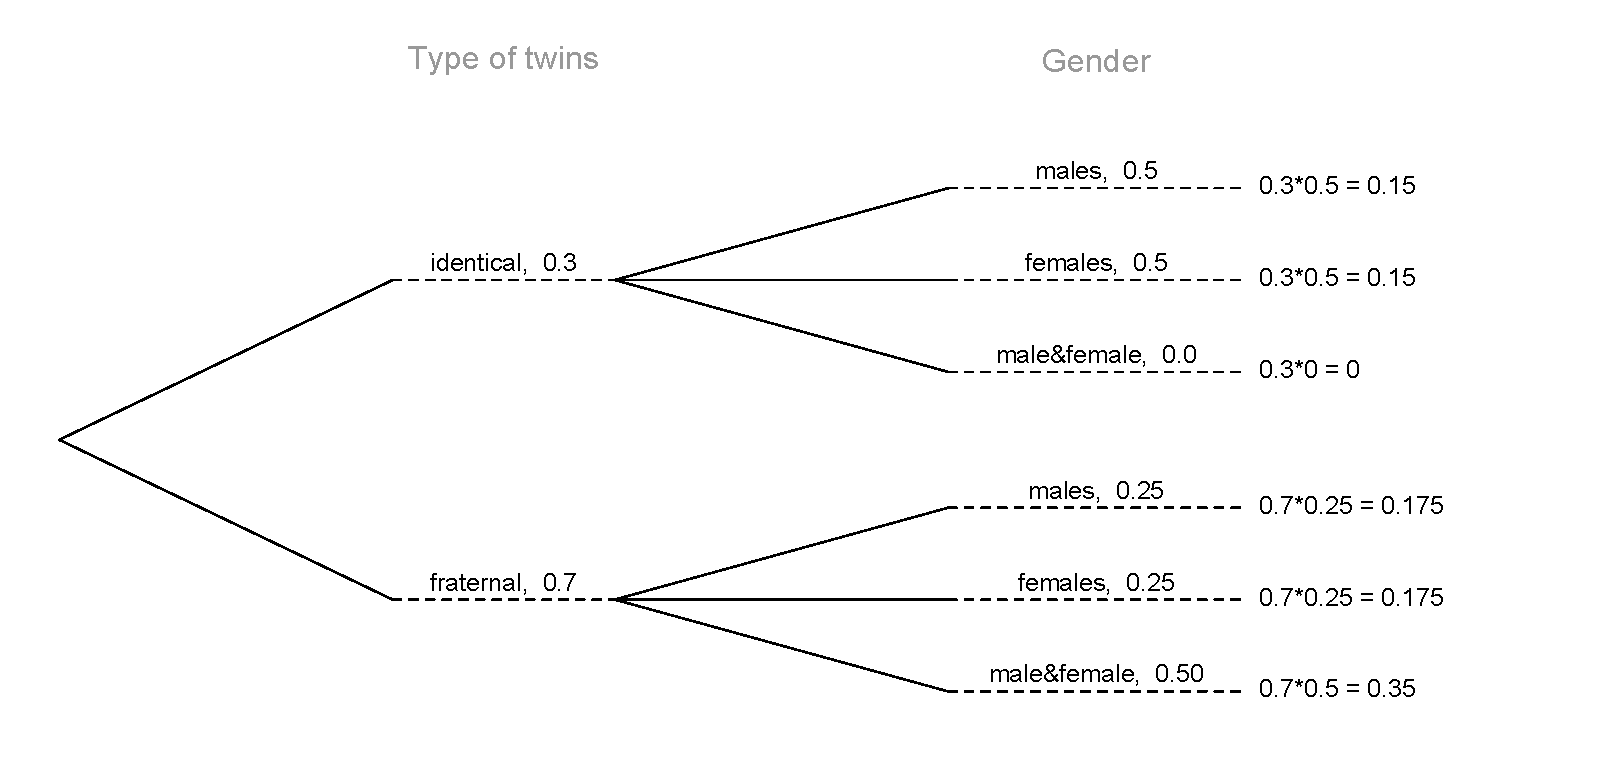
\includegraphics[width = 0.9\textwidth]{figures/twins_tree}
\end{center}
}

%

\item \type{CLT - means} Twenty-year-old men's weights have a population mean of 155 pounds and a population standard deviation of 22 pounds (www.kidsgrowth.com). The distribution is right-skewed. Suppose we take a random sample of 100 twenty-year-old men's weights.\footnote{Adapted from \textit{Introductory Statistics} by Gould and Ryan.}

\begin{enumerate}

\item Explain why the Central Limit Theorem is applicable.

\soln{The sample is random and less than 10\% of all twenty-year-old men, hence the observations are independent. The population distribution is not normal, but since the sample size is greater than 30, we can assume the sampling distribution will be nearly normal.}

\item Sketch the sampling distribution of means. Label the mean, the mean $\pm$ 1, 2, and 3 standard errors, and indicate what percent of the distribution falls in each region.

\soln{
\[ \bar{x} \sim N \left( mean = \mu, SE = \frac{s}{\sqrt{n}} \right) = N \left( mean = 155, SE = \frac{22}{\sqrt{100}} = 2.2 \right) \]
\begin{align*}
155 \pm 1 * 2.2 &= (152.8, 157.2) \\
155 \pm 2 * 2.2 &= (150.6, 159.4) \\
155 \pm 3 * 2.2 &= (148.4, 161.6) \\
\end{align*}
\begin{center}
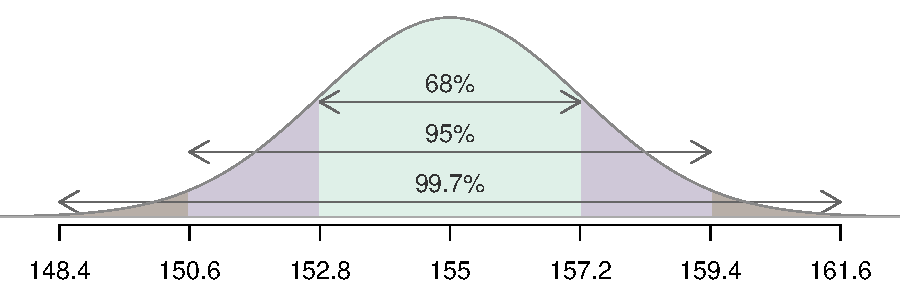
\includegraphics[width=0.65\textwidth]{figures/menweights}
\end{center}
}

\item What percent of random samples of 100 twenty-year-old men have means between 150.6 and 161.6 pounds?

\soln{Lower end = 100 - 95 = 5 / 2 = 2.5\% \\
Upper end = 100 - 99.7 = 0.3 / 2 = 0.15\% \\
Middle = 100 - (2.5 + 0.15) = 97.35\%}

\end{enumerate}

%

\item \type{CLT - proportions} It is believed that nearsightedness affects about 8\% of all children. Would it be considered unusual if 21 our of 194 randomly sampled children are nearsighted? Explain your reasoning.

\soln{First we need to find the expected proportion of nearsighted children in this group, and its standard error.
\[ \hat{p} \sim N \left( mean = p = 0.08, SE = \sqrt{\frac{p(1-p)}{n}} = \sqrt{\frac{0.08 * 0.92}{194}} = 0.0195 \right) \]
A sample proportion within two standard deviations of the mean would not be considered unusual.
\[ 0.08 \pm 2 * 0.0195 = (0.041, 0.119) \]
The observed sample proportion is $21 / 194 = 0.108$, which is within the usual range, so not unusual.
}

%

\item \type{Means - one large sample} A clinical trial with 400 subjects was conducted to test whether the average weight loss using a new diet pill is significant. You know that the standard deviation of the test subject's weight loss was 5lbs. Give an example of sample mean weight loss which would result in rejecting the null hypothesis at the 5\% level but not rejecting it at the 1\% level. Hint: We only care if the subjects lost weight and not gained it, think about what tails are appropriate and start by writing the appropriate hypotheses.

\soln{The hypotheses are:
\begin{itemize}
\item[] $H_0: \mu_{diff} = 0$
\item[] $H_0: \mu_{diff} > 0$
\end{itemize}
In order to reject the hypothesis at the 5\% significance level we would need a Z-score of 1.65 or higher.
\begin{center}
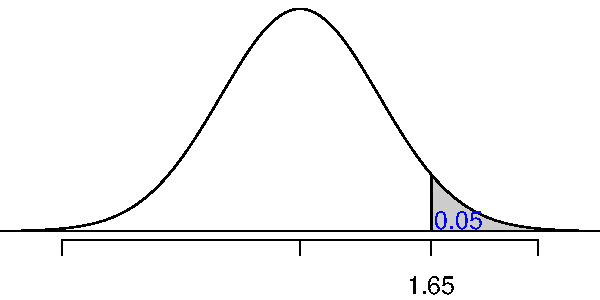
\includegraphics[width=0.45\textwidth]{figures/z95}
\end{center}
Using the following we can calculate the minimum required $\bar{x}$ to reject $H_0$ at 5\% significance level.
\[ 1.65 = \frac{\bar{x} - 0}{\frac{5}{\sqrt{400}}} \rightarrow \bar{x} = 1.65 * \frac{5}{\sqrt{400}} = 0.4125  \]
Next, we need to figure out the required Z-score for significance at 1\% level.
\begin{center}
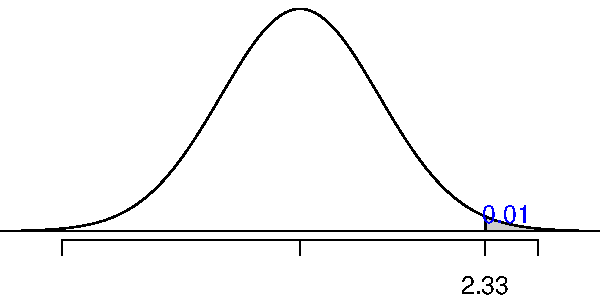
\includegraphics[width=0.45\textwidth]{figures/z99}
\end{center}
Using the following we can calculate the minimum required $\bar{x}$ to reject $H_0$ at 5\% significance level.
\[ 2.33 = \frac{\bar{x} - 0}{\frac{5}{\sqrt{400}}} \rightarrow \bar{x} = 2.33 * \frac{5}{\sqrt{400}} = 0.5825  \]
So average weight loss between 0.4125 pounds and 0.5825 pounds will result in rejecting $H_0$ at 5\% significance level but not at 1\% significance level.
}

%

\item \type{Means - two large samples} In June 2002, the \textit{Journal of Applied Psychology} reported on a study that examined whether the content of TV shows influenced the ability of viewers to recall brand names of items featured in the commercials. The researchers randomly assigned volunteers to watch one of three programs, each containing the same nine commercials. One of the programs had a violent content, another sexual content, and the third neutral content. After the shows ended, the subjects were asked to recall the brands of products what were advertised. Results are summarized in the table below.\footnote{Adapted from \textit{Intro Stats}, by De Veaux, Velleman, and Bock.}
\begin{center}
\begin{tabular}{l | c | c | c |}
					& \multicolumn{3}{c |}{\textit{Program Type}} \\
\cline{2-4}
					& Violent	& Sexual	& Neutral	\\	
\hline	
No. of subjects			& 101	& 106	& 103	\\
\hline
\textit{Brands recalled}	&		&		& \\
\hspace{5mm} Mean		& 3.02	& 2.72	& 4.65 \\
\hspace{5mm} SD		& 1.61	& 1.85	& 1.62 \\
\end{tabular}
\end{center}

For the following questions, you may assume that all assumptions and conditions necessary for inference are satisfied.
\begin{enumerate}
\item Is there a significant difference in viewers' abilities to remember brands advertised in shows with \textbf{violent} vs. \textbf{neutral} content? Use a hypothesis test to answer this question and make sure to interpret your conclusion in context.

\soln{Let violent be group 1 and sexual be group 2. \\
$H_0: \mu_{v} = \mu_{n}$ \\
$H_A: \mu_{v} \ne \mu_{n}$\\
\[ Z = \frac{\bar{x}_{v} - \bar{x}_{n}}{\sqrt{\frac{s_v^2}{n_v} + \frac{s_n^2}{n_n}}} = \frac{3.02 - 4.65}{\sqrt{\frac{1.61^2}{101} + \frac{1.62 ^2}{103}}} = \frac{-1.63}{0.22615} = -7.21  \]
\[ p-value \approx 0 \]
Since p-value $<$ 0.05, we reject $H_0$. There is convincing evidence to suggest a difference in viewers' abilities to remember brands advertised in shows with violent vs. neutral content.
}

\item Construct a 95\% confidence interval for the difference in number of brand names recalled between the groups watching shows with \textbf{sexual} content and those watching \textbf{neutral} shows. Interpret your interval in context.

\soln{
\begin{align*}
(\bar{x}_s - \bar{x}_n) \pm z^* \sqrt{\frac{s_s^2}{n_s} + \frac{s_n^2}{n_n}} &= (2.72 - 4.65) \pm 1.96 *  \sqrt{\frac{1.85^2}{106} + \frac{1.62^2}{103}} \\
&= -1.93 \pm 1.96 * 0.24 \\
&= -1.93 \pm 0.47 \\
&= ( -2.4, -1.46)
\end{align*}
We are 95\% confident that the average number of brand names recalled after watching shows with sexual content is 2.4 to 1.46 lower than the average number brands recalled after watching shows with neutral content.
}

\item What type of test would we use if we wanted to compare all three means simultaneously.

\soln{ANOVA - F-test.}

\end{enumerate}

%

\item \type{Means - one small sample} Cedar-apple rust is a (non-fatal) disease that affects apple trees. Its most obvious symptom is rust-colored spots on apple leaves. Red cedar trees are the immediate source of the fungus that infects the apple trees. If you could remove all red cedar trees within a few miles of the orchard, you should eliminate the problem. In the first year of an experiment the number of affected leaves on 8 randomly sampled trees were counted; the following winter all red cedar trees within 100 yards of the orchard were removed and the following year the same trees were examined for affected leaves. The results are recorded below:\footnote{Adapted from http://www.physics.csbsju.edu/stats/t-test.html}

\begin{center}
{\small
\begin{tabular}{r | c c | c}
tree	& number of rusted	& number of rusted	& difference \\
	& leaves: year 1	& leaves: year 2      	& year 1 -  year 2 \\
\hline
  1   &        38        &          32       &       6      \\
  2   &         10       &           16      &       -6 \\
  3   &         84       &           57      &       27 \\
  4   &         36       &           28      &        8 \\
  5   &        50        &          55       &      -5 \\
  6   &         35       &           12      &       23 \\
  7   &        73        &          61       &      12 \\
  8   &       48         &         29        &     19 \\
\hline
average     &   46.8          &       36.2       &      10.5 \\
standard dev  &  23 &                  19  &              12
\end{tabular}
}
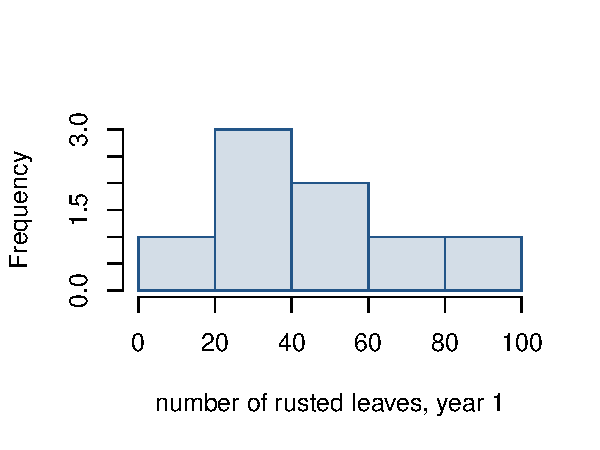
\includegraphics[width = 0.45\textwidth]{figures/year1}
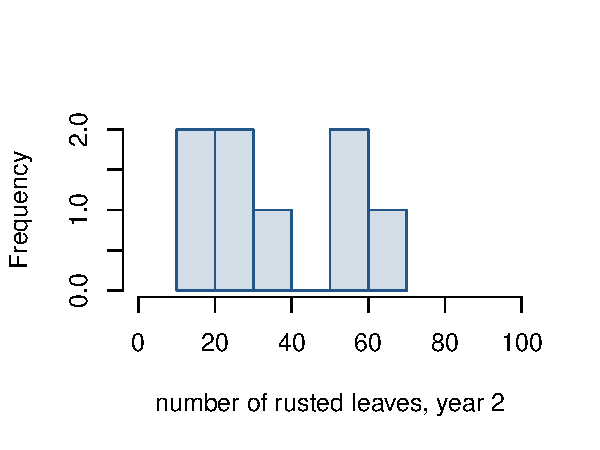
\includegraphics[width = 0.45\textwidth]{figures/year2}
\end{center}

\begin{enumerate}

\item Write the hypotheses for testing for a difference between the average number of rusted leaves between years 1 and 2.

\soln{$H_0: \mu_{diff} = 0$ \\
$H_A: \mu_{diff} \ne 0$}

\item Check the assumptions and conditions necessary for inference and determine the most appropriate statistical method for evaluating these hypotheses.

\soln{The sample is random and likely less than 10\% of all trees, hence we can assume that the number of rusted leaves on one tree in the sample is independent of another. The distributions for number of rusted leaves in years 1 and 2 do not appear to be extremely skewed, so the distribution of the difference is not either. Since the sample size is small $n < 30$ we use a T-test. And since the two samples are dependent, we do a paired test.}

\item Calculate the test statistic and the p-value.

\soln{\[ T = \frac{10.5 - 0}{\frac{12}{\sqrt{8}}} = 2.47, \quad df = 8 - 1 = 7, \quad 0.02 < p-value < 0.05 \]}

\item What is the conclusion of the hypothesis test?

\soln{Since p-value is less than 5\% we reject $H_0$. The data provide convincing evidence that the average number of rusted leaves has changed between years 1 and 2.}

\item What is the p-value for testing if the number of rusted leaves has \underline{decreased} from year 1 to 2. Give an interpretation of this new p-value.

\soln{The p-value would be half of what we found earlier: $0.01 < p-value < 0.025$. If in fact the average number of rusted leaves has remained the same, the probability of observing a random sample of 8 trees where the average number of rusted leaves has decreased by 10.5 or more is between 0.01 and 0.025.}

\end{enumerate}

%

\item \type{Means - two sample randomization} Can a simple smile have an effect on punishment assigned following an infraction? ``Why smiles generate leniency", LaFrance \& Hecht (1995), examines the effect of a smile on the leniency of disciplinary action for wrongdoers. Participants in the experiment took on the role of members of a college disciplinary panel judging students accused of cheating. For each suspect, along with a description of the offense, a picture of one of 34 students was provided. Each student had a picture where they smiled and one where they had a neutral facial expression. A leniency score was calculated based on the disciplinary decisions made by the participants. Suppose the experimenters have prior knowledge that smiling has a positive influence on people, and they are testing to see if the average lenience score is higher for smiling students than it is for students with a neutral facial expression (or, in other words, that smiling students are given milder punishments.) In the original sample the average leniency score for smiling students was 4.912 and for students with a neutral expression was 4.118. The figure below shows the distribution of the difference between the sample means from 1,000 randomization samples.\footnote{Adapted from \textit{Unlocking the Power of Data} by Lock, Lock, Lock, Lock, and Lock.}

\begin{center}
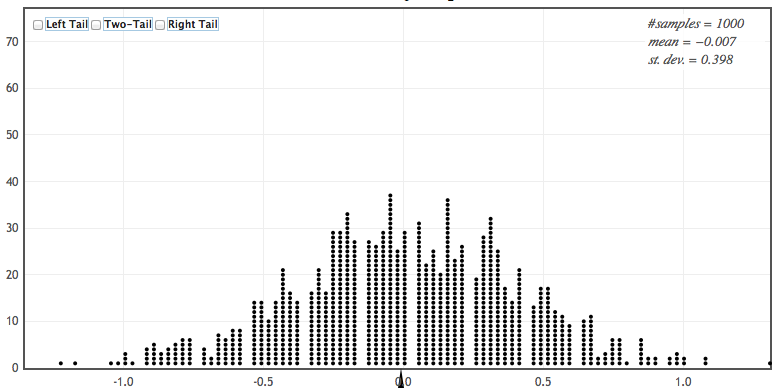
\includegraphics[width = \textwidth]{figures/smiling}
\end{center}

\begin{enumerate}
\item Are the two groups dependent or independent?

\soln{Dependent, it's the same student's picture.}

\item Write the appropriate hypotheses.

\soln{Let $\mu_{diff}$ represent the average difference between the leniency scores for smiling - neutral students. \\
$H_0: \mu_{diff} = 0$ \\
$H_A: \mu_{diff} > 0$}

\item What is the conclusion of the hypothesis test?

\soln{The p-value is roughly 20 / 1000 = 0.02. With a low p-value we reject $H_0$. The data provide convincing evidence to suggest that students who smile in their pictures have higher leniency scores than those who have a neutral expression.}

\end{enumerate}

%

%

%\item \type{Proportions - one large sample} In November 2009, 11\% of Americans thought the country representing ``greatest danger" to the US was China.  In Jan 2011, a survey conducted by the Pew Research Foundation showed that out of the 1,503 randomly sampled Americans 20\% agree with that statement. Do these data provide convincing evidence that the proportion of Americans who think China is the greatest danger to the US has increased over the last couple years? Conduct a hypothesis test to answer this question and also interpret the p-value in context of the question.
%
%\soln{
%\begin{align*}
%H_0&: p = 0.11 \text{ (The true population proportion of Americans who think China is }\\
%&\text{the greatest danger to the US is still 11\%, the observed statistic of 20\% was simply} \\
%&\text{due to chance.)}\\
%H_A&: p > 0.11 \text{ (The true population proportion of Americans who think China is the} \\
%&\text{greatest danger to the US has increased over the last couple years, the observed statistic} \\
%&\text{was due to a real increase in the true population proportion.)} \\
%\end{align*}
%Assumptions/conditions:
%\begin{enumerate}[1.]
%\item Independent observations: The sample is random and less than 10\% of the US population, therefore we can assume that the opinion of one sampled individual is independent of another.
%\item Nearly normal: $1503 * 0.11 = 165.33$ and $1503 * 0.89 = 1337.67$ are all greater than 10, therefore the distribution of the sample proportion will be nearly normal.
%\end{enumerate}
%\begin{align*}
%Z &= \frac{obs - mean}{SD} = \frac{0.20 - 0.11}{\sqrt{\frac{0.11*0.89}{1503}}} = \frac{0.20 - 0.11}{0.00807} = 11.15 \\
%p-value &= P(\hat{p} > 0.20~|~p = 0.11) = P(Z > 11.15) \approx 0
%\end{align*}
%The data provide convincing evidence that the proportion of Americans who think China is the greatest danger to the US has increased over the last couple years. \\
%Interpretation of the p-value: If in fact 11\% of Americans think that China is the greatest danger to the US, the probability of getting a random sample of 1,503 Americans where 20\% or more think so would be almost 0.
%}

%

\item \type{Proportions - two large samples}A USA Today/Gallup poll conducted between Dec. 21, 2010 - Jan. 9, 2011 asked a group of unemployed and underemployed Americans if they have had major problems in their relationships with their spouse or another close family member as a result of not having a job (if unemployed) or not having a full-time job (if underemployed). 1,145 unemployed and 675 underemployed people were randomly sampled and surveyed. 27\% of the unemployed and 25\% of the underemployed people said they had major problems in relationships as a result of their employment status. 

\begin{enumerate}

\item Are conditions for inference satisfied?

\soln{\begin{enumerate}[1.]
\item Independent observations: Since both conditions are satisfied we can assume that unemployed people in the sample are independent of one another and the underemployed people in the sample are also independent of one another (with respect to having problems in relations).
\begin{itemize}
\item Randomization condition: We are told that both samples are random. 
\item 10\% Condition:  1145 $<$ 10\% of all unemployed and 675 $<$ 10\% of all underemployed
\end{itemize}
\item Nearly normal condition:  Since S/F condition is met, we can assume that the difference between the two sample proportions are distributed nearly normally.
\begin{align*}
1145 * 0.27 = 309.15 > 10~&\hspace{1cm}~675 * 0.25 = 168.75 > 10 \\
1145 * 0.73 = 835.85 > 10~&\hspace{1cm}~675 * 0.75 = 506.25 > 10
\end{align*}
\item Independent groups :  Since the samples are random we have no reason to believe the two groups are not independent of each other.
\end{enumerate}
}

\item Construct a 95\% confidence interval to estimate the difference between the true population proportions of unemployed and underemployed people who had such problems.

\soln{The confidence interval can be calculated as follows:
\begin{align*}
(\hat{p}_{unemp} - \hat{p}_{underemp}) &\pm z^* \sqrt{\frac{\hat{p}_{unemp} (1 - \hat{p}_{unemp})}{n_{unemp}} + \frac{\hat{p}_{underemp} (1 - \hat{p}_{underemp})}{n_{underemp}}} \\
(0.27 - 0.25) &\pm 1.96 * \sqrt{\frac{0.27 * 0.73}{1145} + \frac{0.25 * 0.75}{675}} \\
0.02 &\pm 1.96 * 0.0212 \\
0.02 &\pm 0.04 \\
(-0.02&, 0.06)
\end{align*}
We are 95\% confident that the proportion of unemployed people who had problems in relationships are 2\% lower to 6\% higher than the proportion of underemployed people who had such issues.}

\item Conduct a hypothesis test to evaluate if these data provide convincing evidence to suggest a difference between the true population proportions of unemployed and underemployed people who had such problems. Use a 5\% significance level.

\soln{\begin{align*}
H_0&: p_{unemp} = p_{underemp} \\
H_A&: p_{unemp} \ne p_{underemp} \\
\end{align*}
The pooled proportion is
\[ \hat{p} = \frac{suc_1 + suc_2}{n_1 + n_2} = \frac{1145 * 0.27 + 675 * 0.25}{1145 + 675} = 0.26 \]
We should re-check the conditions to make sure with the pooled proportion expected successes and failures will be at least 10, but since sample sizes are large and the pooled proportion is not much different than the sample proportions, we can be fairly certain that the condition is met. \\
The test statistic and p-value are
\begin{align*}
Z &= \frac{(\hat{p}_1 - \hat{p}_2) - 0}{\sqrt{\frac{\hat{p} \hat{q}}{n_1} + \frac{\hat{p} \hat{q}}{n_2}}} = \frac{(0.27 - 0.25)}{\sqrt{\frac{0.26 * 0.74}{1145} + \frac{0.26 * 0.74}{675}}} = \frac{0.02}{0.0213} = 0.94 \\
p-value &= 2 * (1 -  0.826) = 0.3472
\end{align*}
Since the p-value is so large, we fail to reject $H_0$. The data do not provide convincing evidence that the true population proportions of unemployed and underemployed people who had major problems in relationships due to their employment status are different. The observed difference between the sample proportions was simply due to chance.}

\end{enumerate}

%

\item \type{Chi-square - GOF} As recently as 2008, 70\% of users of social networking sites such as Facebook were 35 years old or younger. Now the age distribution is much more spread out. The table below shows the age distribution of 975 users of social networking sires from a  Pew Research survey from June 2011.\footnote{From \textit{Unlocking the Power of Data} by Lock, Lock, Lock, Lock, and Lock.}

\begin{center}
\begin{tabular}{l | c | c | c | c | c}
Age			& 18 - 22	& 23 - 35 	& 36 - 49 	& 50 - 65 	& 65 + \\
\hline
Frequency	& 156 	& 312	& 253	& 195	& 59 \\
\end{tabular}
\end{center}

\begin{enumerate}[(a)]
\item Test an assumption that users are equally likely to be in each of the five age groups listed. Show all details of the test.

\soln{$H_0$: Users are equally likely to be in each of the five groups listed. \\
$H_A$: Users are not equally likely to be in each of the five groups listed. \\
The total number of users in the study is  $156 + 312 + 253 + 195 + 59 = 975$. If the distribution was uniform across all categories we would expect to see $975 / 5 = 195$ users in each category. \\
The chi-squared statistic, the degrees of freedom associated with it, and the p-value can be calculated as follows:
\begin{align*}
\chi^2 &= \sum \frac{(O - E)^2}{E} \\
&=  \frac{(156 - 195)^2} {195} + \frac{(312 - 195)^2} {195} + \frac{(253 - 195)^2} {195} + \frac{(195 - 195)^2}{195} + \frac{(59 - 195)^2}{195} = 190.1026 \\
df &= k - 1 = 5 - 1 = 4 \\
p-value &< 0.001
\end{align*}
With such a small p-value we reject $H_0$. The data provide convincing evidence that users are not equally likely to be in each of the five groups listed.}

\item Which age group contributes the largest amount to the test statistic? For the age group, is the observed count smaller or larger than the expected count?

\soln{The 65+ age group has the largest contribution to the sum for the test statistic. The observed count is much smaller than expected.}

\end{enumerate}

%

%\item \type{Chi-square - independence} ``Further observations on the manner of clasping the hands", Downey (1926), found 190 right-thumb and 149 left-thumb-claspers among right-handed women, and 42 right-thumb and 49 left-thumb-claspers among left-handed women.\footnote{Adapted from \textit{Handbook of Biological Statistics} by McDonald.} 
%
%\begin{minipage}[b]{0.70\textwidth}
%\begin{enumerate}[(a)]
%\item Make a contingency table summarizing the data.
%\item Use a $\chi^2$ statistics to evaluate if handedness and choice of \\ thumb are related.
%\vspace{2.5cm}
%\end{enumerate}
%\end{minipage}
%\begin{minipage}[b]{0.25\textwidth}
%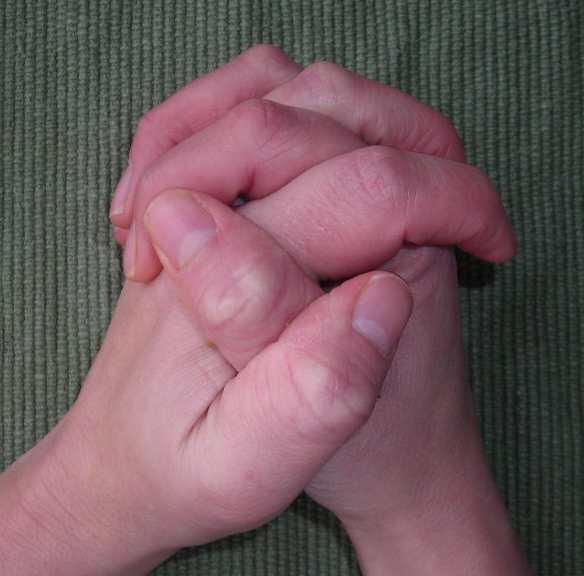
\includegraphics[width=\textwidth]{figures/clasp}
%\end{minipage}
%
%\soln{
%\begin{enumerate}[(a)]
%\item The contingency table is shown below:
%\begin{center}
%\begin{tabular}{l | c | c | c}
%			& Right thumb	& Left  thumb 	& Total	 \\
%\hline
% Right-handed 	& 190 		& 149		& 339 \\
% Left-handed	& 42			& 49 			& 91\\
% \hline
% Total		& 232		& 198		& 430
%\end{tabular}
%\end{center}
%\item 
%$H_0$: Handedness and choice of thumb are independent. \\
%$H_A$: Handedness and choice of thumb are associated. \\
%The contingency table below shows the expected counts for each cell:
%\begin{center}
%\renewcommand{\arraystretch}{1.5}
%\begin{tabular}{l | c | c | c}
%			& Right thumb	& Left  thumb 	& Total	 \\
%\hline
% Right-handed 	& $\frac{339 * 232}{430} = 183$ 		&  $\frac{339 * 198}{430} = 156$ 		& 339 \\
% Left-handed	& $\frac{91 * 232}{430} = 49$			& $\frac{91 * 198}{430} = 42$  			& 91\\
% \hline
% Total		& 232		& 198		& 430
%\end{tabular}
%\end{center}
%The chi-squared statistic, the degrees of freedom associated with it, and the p-value can be calculated as follows:
%\begin{align*}
%\chi^2 &= \sum \frac{(O - E)^2}{E} \\
%&=  \frac{(190 - 183)^2} {183} + \frac{(149 - 156)^2} {156}  + \frac{(42 - 49)^2}{49} + \frac{(49 - 42)^2}{42} = 2.75 \\
%df &= (R - 1) * (C - 1) = 1 \\
%0.05 &< p-value < 0.1
%\end{align*}
%p-value $>$ 0.05, so we fail to reject $H_0$. The data do not provide convincing evidence that handedness and choice of thumb are associated.
%\end{enumerate}
%}

%

\item \type{Proportion - two large sample CI via bootstrapping} A random sample of 3,052 cell phone users were asked ``Do you send or receive text messages on your cell phone?" Of the 800 teens 696 said they did, and of the 2252 adults 1621 said they did. The histogram below shows the bootstrap distribution for the difference between the proportions of teens and adults who send or receive text messages on their cell phones. The plot below shows the distribution for the difference between the proportions of teens and adults ($\hat{p}_{teen} - \hat{p}_{adult}$) in 10,000 \textbf{bootstrap} samples.\footnote{Adapted from \textit{Unlocking the Power of Data} by Lock, Lock, Lock, Lock, and Lock.}

\begin{minipage}[c]{0.40\textwidth}
\begin{enumerate}
\item Estimate the mean of the bootstrap distribution.
\item Which of the below is the most reasonable estimate of the standard error of the difference in proportions? Explain your reasoning for your choice.
\begin{multicols}{2}
\begin{enumerate}[(a)]
\item 0.015
\item 0.03
\item 0.05
\item 0.15
\end{enumerate}
\end{multicols}
\item Using your choice for SE in part (b), find an interval estimate for the difference in proportions of teen and adult cell phone users who send/receive text messages.
\end{enumerate}
\end{minipage}
\begin{minipage}[c]{0.50\textwidth}
\begin{center}
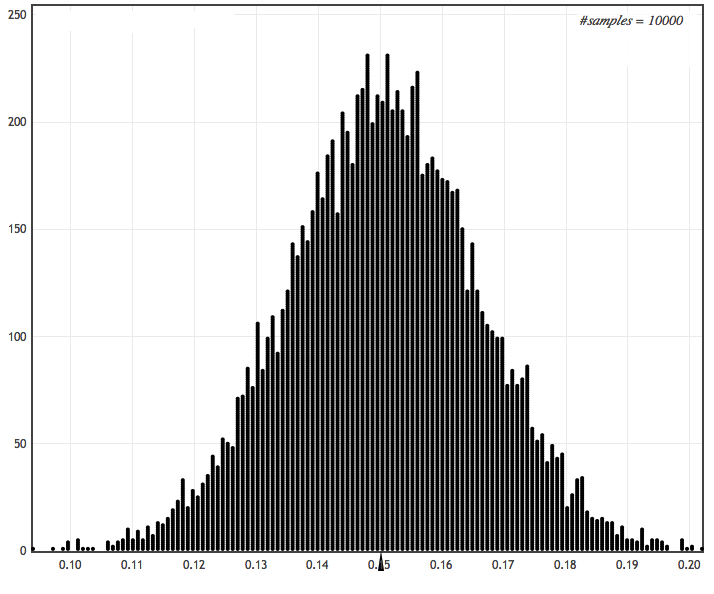
\includegraphics[width = \textwidth]{figures/texting}
\end{center}
\end{minipage}

\soln{
\begin{enumerate}
\item The mean of the bootstrap distribution is 0.15, this is the center of the distribution as well as the difference between the observed sample proportions ($\frac{696}{800} - \frac{1621}{2252} = 0.87 - 0.72 = 0.15$)
\item 0.015 - the distribution spans about 6 SEs, 3 below and 3 above the mean. The other options are too large.
\item $0.15 \pm 2 * 0.015 = (0.12, 0.18)$ - We are 95\% confident that the proportion of teens who send/receive texts is 12\% to 18\% higher than the proportion of adults who do.
\end{enumerate}
}

%

\item \type{Proportion - one large sample CI, determine n} In a state where the political race is tight you have the job of conducting a survey on a simple random sample of voters from the state to determine who has the edge. As a pollster, you know that to give your poll credit, you need to ensure the estimate is within 4 percentage points (with 99\% confidence). Determine the minimum sample size that will ensure this accuracy.
\soln{\[ 0.04 = 2.58\sqrt{\frac{0.5 * 0.5}{n}} \rightarrow n = \frac{2.58^2 * 0.5 * 0.5}{0.04^2} = 1040.062 \rightarrow n \ge 1041 \]}


%

\item \type{SLR} The mean fat content of the 30 Burger King menu items is 23.5g with a standard deviation of 16.4g, and the mean protein content of these items is 17.2g with a standard deviation of 14g. If the correlation between protein and fat contents is 0.83. A scatterplot of the data is shown below.

\begin{center}
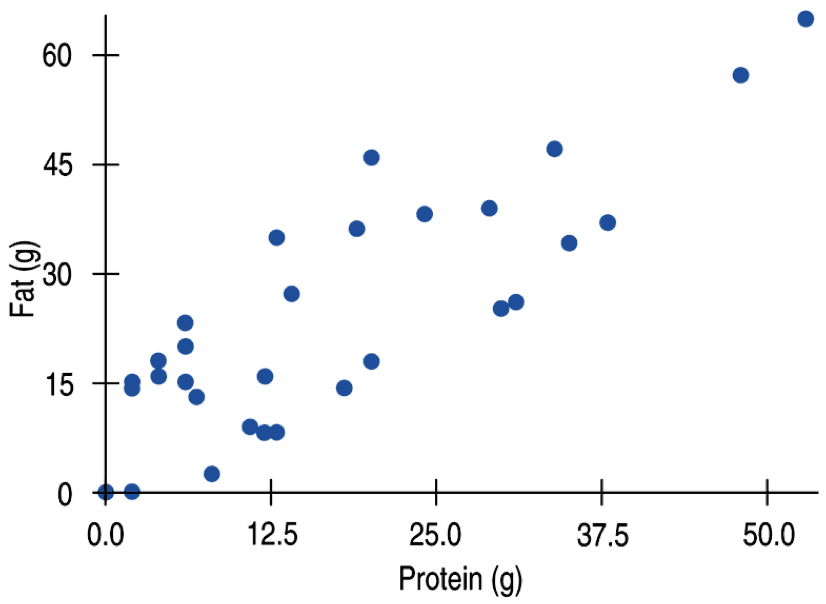
\includegraphics[width=0.5\textwidth]{figures/burgerking}
\end{center}

\begin{enumerate}

\item Write the linear model for predicting fat content.
\soln{
\begin{align*}
slope &= r \frac{s_y}{s_x} = 0.83 * \frac{16.4}{14} = 0.97 \\
intercept &= \bar{y} - b \bar{x} = 23.5 - 0.97 * 17.2 = 6.8 \\
\widehat{fat} &= 6.8 + 0.97 * protein
\end{align*}
}

\item Interpret the slope and the intercept in context.
\soln{
\begin{itemize}
\item For one gram increase in protein content, we would expect the fat content to increase on average by 0.97 grams.
\item Burger King menu items with no protein are expected to have a fat content of 6.8 grams. It is unlikely that such a food item exists, so the intercept might not make sense in context.
\end{itemize}
}

\item A new BK menu item has 30 grams of protein. Can we use this model to predict its fat content? If so, what is it?

\soln{The predicted fat content for a BK Broiler chicken sandwich is $6.8 + 0.97 * 30 = 35.9$ grams.}

\item Another new BK menu item has 75 grams of protein. Can we use this model to predict its fat content? If so, what is it?

\soln{We should not use the linear model to predict the amount of fat in a burger with 75 grams of protein since the data we used to create the model is for burgers with approximately 0 to 50 grams of protein.}

\item Based on the residuals plot shown below, does the linear model appear to be appropriate for these data?

\begin{center}
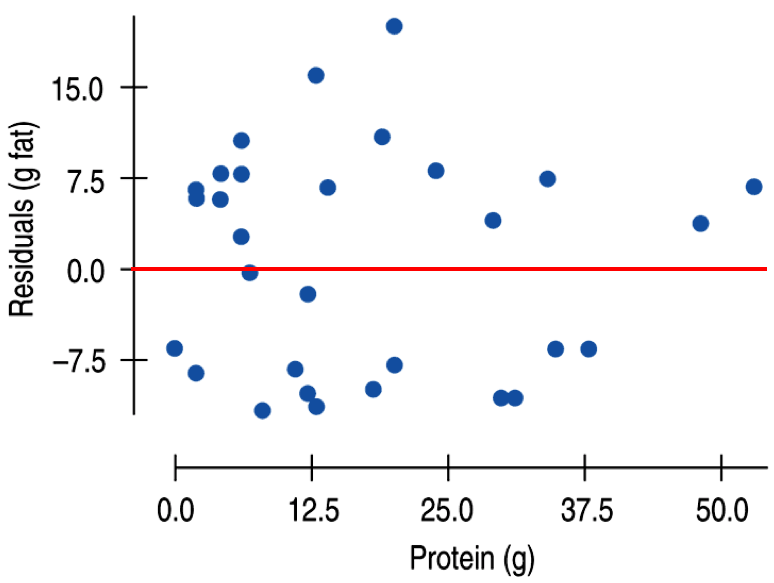
\includegraphics[width=0.5\textwidth]{figures/burgerking_resvsx}
\end{center}

\soln{The residuals for the BK menu regression look randomly scattered around 0, so yes, the model seems to be a good fit.}

\item Calculate $R^2$ and interpret it in context.

\soln{$R^2 = 0.83^2 = 0.69$. 69\% of the variation in fat content is accounted for by the model, i.e. explained by the protein content of the burger.}

%\item Using the $R^2$ you calculated in part (f), calculate the standard deviation of residuals.
%
%\soln{
%\[ R^2 = 1 - \frac{Var(e)}{Var(y)} \]
%\[0.69 = 1 - \frac{Var(e)}{16.4^2} \rightarrow  \frac{Var(e)}{16.4^2}  = 0.31 \rightarrow Var(e) = 16.4^2 * 0.31 = 83.38 \rightarrow SD(e) = \sqrt{83.38} = 9.13  \]
%}

\end{enumerate}

%

\item \type{MLR} Data was collected on nave heights (ft) and total lengths (ft) of 25 English medieval cathedrals (excerpt shown below).

\begin{minipage}[c]{0.6\textwidth}
\begin{center}
\begin{tabular}{l c c c }
 &  & nave& total \\ 
name & style & height & length \\ 
  \hline
Durham & roman & 75.00 & 502.00 \\ 
  Canterbury & roman & 80.00 & 522.00 \\ 
\vdots \\
  Old St Paul & gothic & 103.00 & 611.00 \\ 
  Salisbury & gothic & 84.00 & 473.00 \\ 
   \hline
\end{tabular}
\end{center}
\end{minipage}
\begin{minipage}[c]{0.4\textwidth}
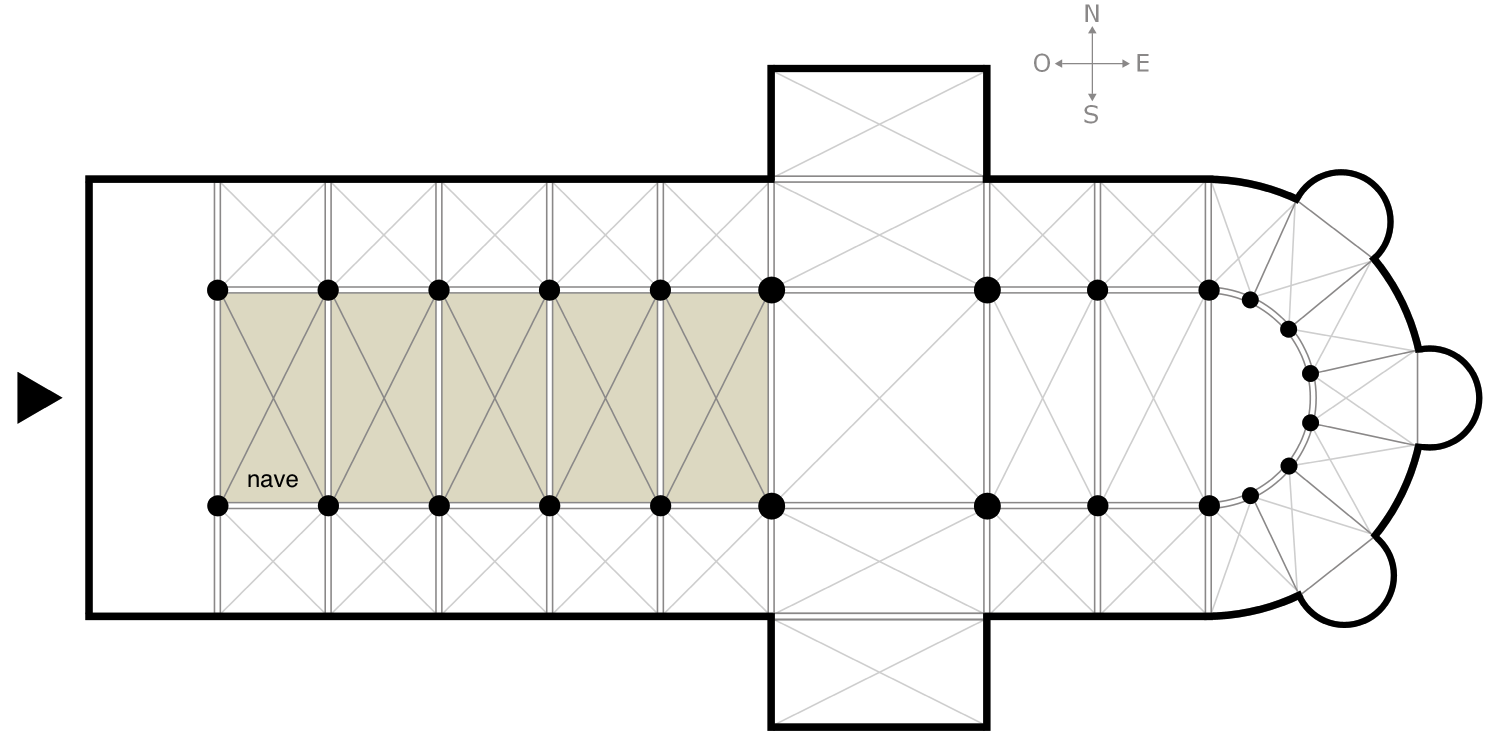
\includegraphics[width=\textwidth]{figures/nave}
\end{minipage}

\begin{enumerate}

\item The regression model for predicting total length from name height and style is also given below. Which of the following is false?
\begin{center}
\begin{tabular}{rrrrr}
  \hline
 & Estimate & Std. Error & t value & Pr($>$$|$t$|$) \\ 
  \hline
(Intercept) & 44.2979 & 81.6477 & 0.54 & 0.5929 \\ 
  naveheight & 4.7116 & 1.0584 & 4.45 & 0.0002 \\ 
  style\_roman & 80.3925 & 32.3063 & 2.49 & 0.0209 \\ 
   \hline
$R^2_{adj} = 49.64\%$ \\
\end{tabular}
\end{center}

\begin{enumerate}[(A)]
\item Each additional foot in nave height is associated with a 4.7116 foot increase in total length.
\item \solnMult{Roman cathedrals with 0 nave height are expected on average to be 44.2979 feet in total length.} 
\item Roman cathedrals are expected on average to be 80.3925 feet longer than Gothic cathedrals.
\item Both nave height and style of cathedral are significant predictors of total length.
\end{enumerate}

\item Using the plots provided below check if the assumptions and conditions for MLR is satisfied.

\begin{center}
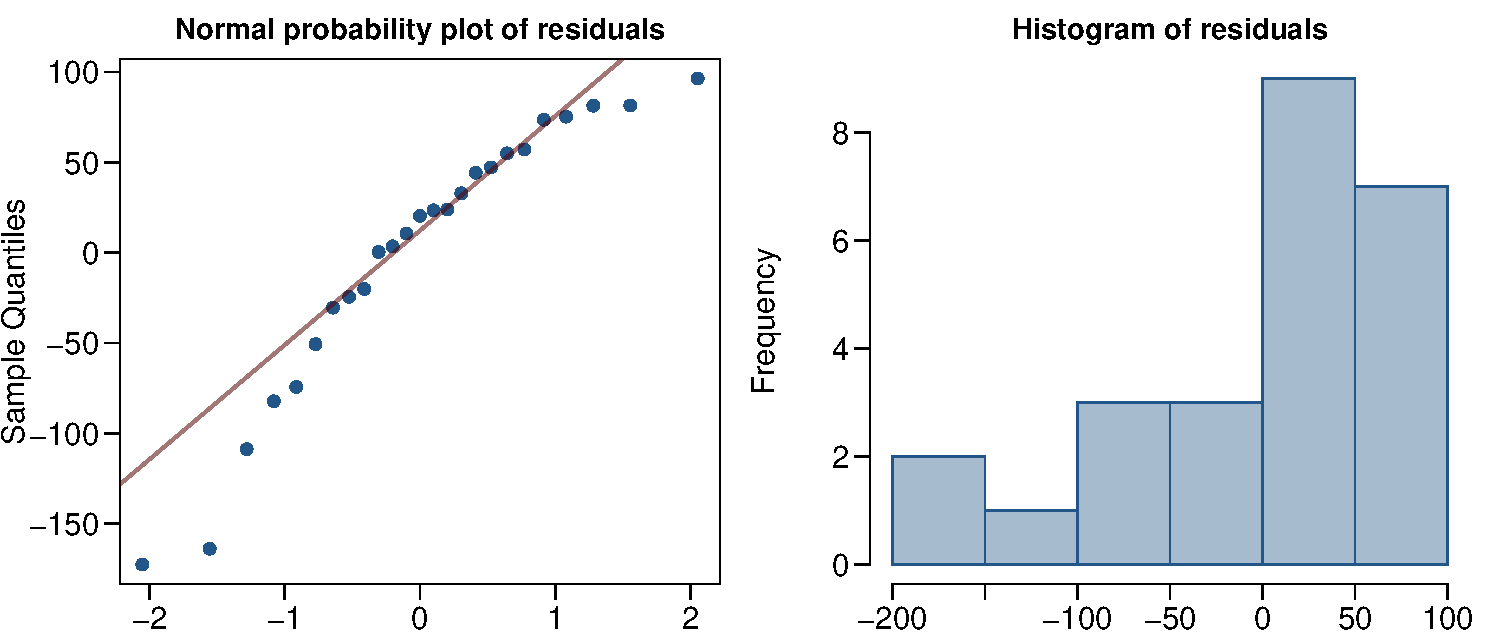
\includegraphics[width=0.7\textwidth]{figures/cath_normal_res}
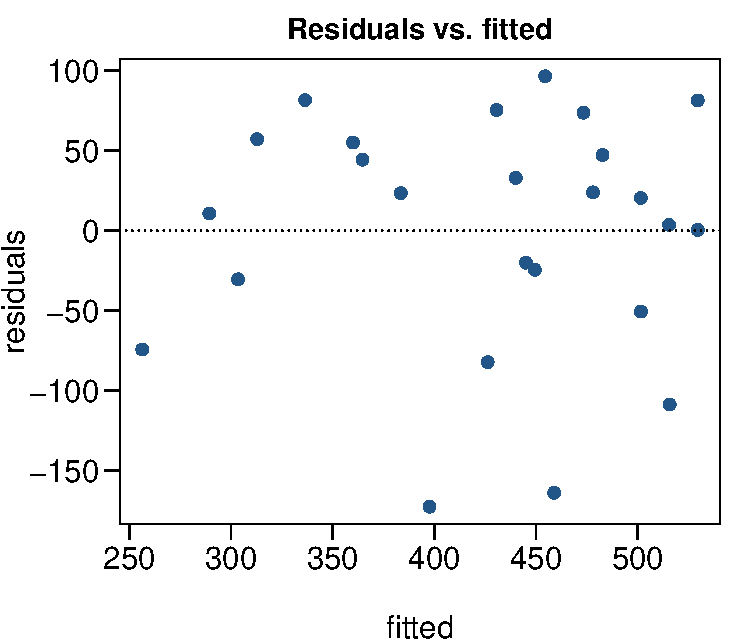
\includegraphics[width=0.35\textwidth]{figures/cath_homo_res}
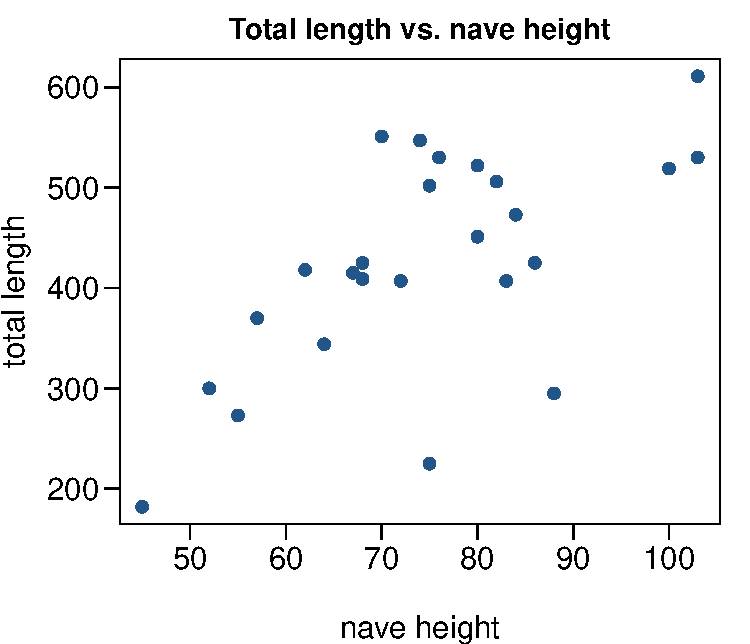
\includegraphics[width=0.35\textwidth]{figures/cath_linear}
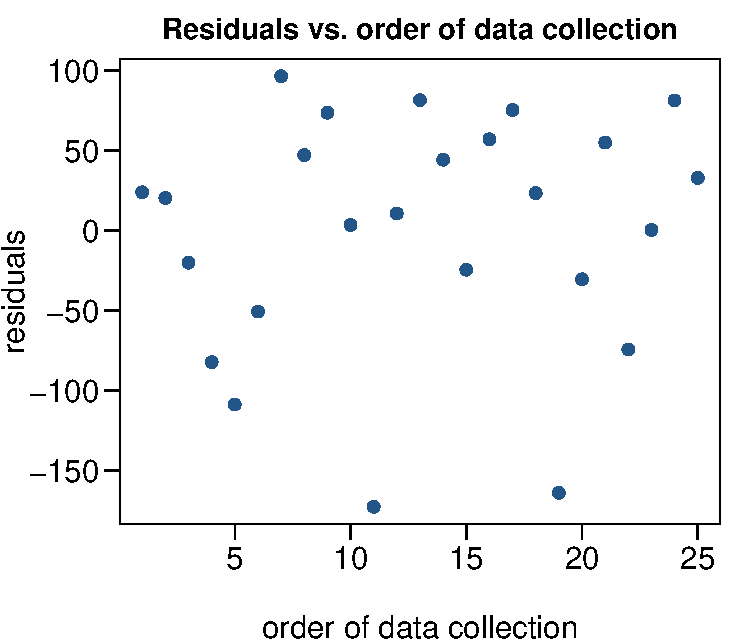
\includegraphics[width=0.35\textwidth]{figures/cath_indep_res}
\end{center}

\soln{\begin{enumerate}[1.]
\item Nearly normal residuals: The residuals appear to have a left-skewed distribution, so this condition is not satisfied.
\item Constant variability in residuals: Residuals vs. fitted plot shows a random scatter so this condition appears to be satisfied.
\item Linearity: The scatterplot of total length vs. nave height shows a somewhat linear relationship, so this condition appears to be satisfied as well.
\item Independent observations: We don't know if the data are sampled randomly but the residuals vs. order of data collection plot shows no apparent trend, hence there is no dependence due to order of data collection.
\end{enumerate}
}

\end{enumerate}

%

\item \type{ANOVA} The Nielsen organization did a poll to determine whether men and women in different age groups watched different amounts of comedy television. The table below shows some summary statistics on each age/gender group.\footnote{Adapted from \textit{Introductory Statistics} by Gould and Ryan.}

\begin{center}
\begin{tabular}{r | c | c | c}
level			& n 	& mean	& sd \\
\hline
men 18-34	& 10	& 287	& 65.05 \\
men 55+		& 10	& 171	& 40.81 \\
women 18-34	& 10	& 353.70	& 20.78 \\
women 55	& 10	& 356.90	& 39.37 \\
\end{tabular}
\end{center}

\begin{enumerate}

\item What method can we use to evaluate if different age/gender groups watch different amounts of comedy television on average. Explain your reasoning.

\soln{ANOVA, comparing means across multiple groups.}

\item Do assumptions and conditions for this technique appear to be satisfied?

\soln{No, there doesn't appear to be constant variance across groups. Standard deviations vary greatly.}

\end{enumerate}

%

\item \type{ANOVA} National Health and Nutrition Examination Survey (NHANES) collects data on people's cholesterol levels and marital status, among many other variables. The data come from 940 respondents and marital status has 6 levels (divorced, living with partner, married, never married, separated, widowed). Below is the relevant ANOVA table.\footnote{Adapted from \textit{Introductory Statistics} by Gould and Ryan.}

\begin{enumerate}

\item Write the hypotheses for evaluating if average cholesterol level varies among people with different marital statuses.

\soln{$H_0: \mu_{D} = \mu_{LWP} = \mu_{M} = \mu_{NM} = \mu_{S} = \mu_{W}$ \\
$H_A:$ At least one pair of means are different.}

\item Below is the relevant ANOVA table. Fill in the blanks.

%\begin{center}
%\begin{tabular}{r c c c c c}
%			& df				& SS			& MS		& F	 & p-value \\
%\hline	
%marital\_st		& \hspace{1cm}	& 89,082		& \hspace{1.5cm}& \hspace{1.5cm} & $<$0.0001	\\
%Residuals		& \hspace{1cm} 	& \hspace{1cm}& \hspace{1.5cm}& 	\\
%\hline	
%Total			& \hspace{1cm}	& 1,909,292 
%\end{tabular}
%\end{center}

\begin{center}
\begin{tabular}{r c c c c c}
			& df				& SS			& MS		& F	 & p-value \\
\hline	
marital\_st		& \soln{6 - 1 = 5}	& 89,082		& \soln{89,082 / 5 = 17,816.4}& \soln{$\frac{17,816.4}{1,948.833} = 9.14$} & $<$0.0001	\\
Residuals		& \soln{934} 	& \soln{1,820,210}  & \soln{1,820,210 / 934 = 1,948.833}& 	\\
\hline	
Total			& \soln{940 - 1 = 939}	& 1,909,292 
\end{tabular}
\end{center}

\item What is the conclusion of the analysis?

\soln{Since p-value is low we reject $H_0$, the data provide convincing evidence that at least one pair of means are different. Cholesterol levels and marital status appear to be associated.}

\item Assuming you did find an association between marital status and cholesterol levels, would this association mean that marital status caused different cholesterol levels? Can you think of a confounding factor?

\soln{No, we can't infer causation based on this study. One possible confounding factor is varying eating habits.}

\end{enumerate}

%

\item \type{CLT} Suppose the true population proportion were $p = 0.1$. The figure below shows what the distribution of a sample proportion looks like when the sample size is $n = 20$, $n = 100$, and $n = 500$. What does each observation in each distribution represent? Describe how the distribution of the sample proportion, $\hat{p}$, changes as $n$ becomes larger.

\begin{center}
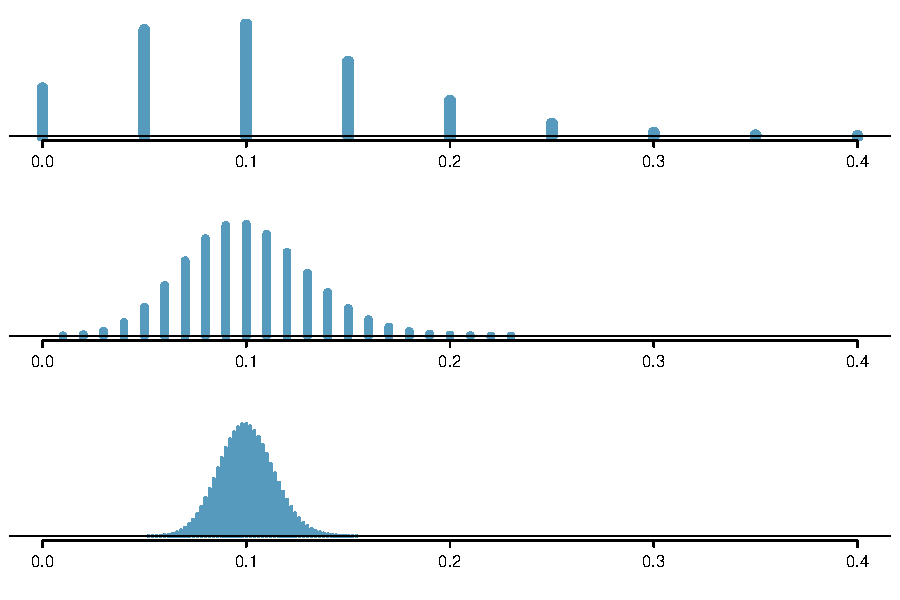
\includegraphics[width = 0.6\textwidth]{figures/eoce-p-hat-simulations-p1}
\end{center}

\soln{Each observation in each of the distributions represents the sample proportion ($\hat{p}$) from samples of size  $n = 20$, $n = 100$, and $n = 500$, respectively. The centers for all three distributions are at 0.10, the true population parameter. When $n$ is small, the distribution is skewed to the right and not smooth. As $n$ increases, the variability of the distribution (standard error) decreases, and the shape of the distribution becomes more unimodal and symmetric.}

%

\item \type{CLT} Suppose the true population proportion were $p = 0.5$. The figure below shows what the distribution of a sample proportion looks like when the sample size is $n = 20$, $n = 100$, and $n = 500$.  What does each observation in each distribution represent? Describe how the distribution of the sample proportion, $\hat{p}$, changes as $n$ becomes larger.

\begin{center}
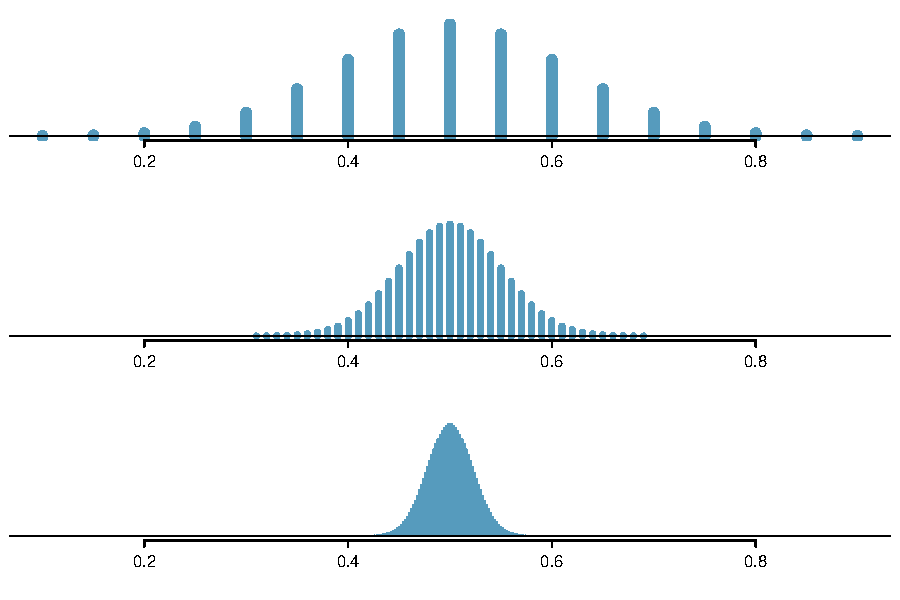
\includegraphics[width = 0.6\textwidth]{figures/eoce-p-hat-simulations-p5}
\end{center}

\soln{Each observation in each of the distributions represents the sample proportion ($\hat{p}$) from samples of size  $n = 20$, $n = 100$, and $n = 500$, respectively. Regardless of the sample size, the shapes of the distributions are symmetric, and centered at 0.50 the true population parameter. However as $n$ increases the variability of the distribution (standard error) decreases.}

%

\item \type{CLT} Suppose the true population proportion were $p = 0.95$. The figure below shows what the distribution of a sample proportion looks like when the sample size is $n = 20$, $n = 100$, and $n = 500$.  What does each observation in each distribution represent? Describe how the distribution of the sample proportion, $\hat{p}$, changes as $n$ becomes larger.

\begin{center}
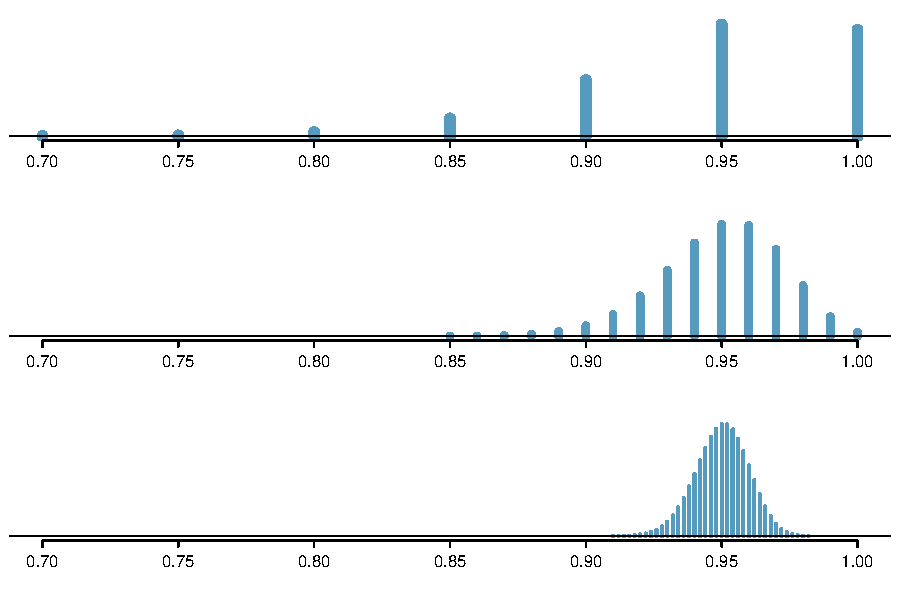
\includegraphics[width = 0.6\textwidth]{figures/eoce-p-hat-simulations-p95}
\end{center}

\soln{Each observation in each of the distributions represents the sample proportion ($\hat{p}$) from samples of size  $n = 20$, $n = 100$, and $n = 500$, respectively. The centers for all three distributions are at 0.95, the true population parameter. When $n$ is small, the distribution is skewed to the left and not smooth. As $n$ increases, the variability of the distribution (standard error) decreases, and the shape of the distribution becomes more unimodal and symmetric.}

%

\item \type{CI}  In 2013, the Pew Research Foundation reported that ``45\% of U.S. adults report that they live with one or more chronic conditions". However, this value was based on a sample, so it isn�t perfect. The study reported a standard error of about 1.2\%, and a normal model may be reasonably be used in this setting. 

\begin{enumerate}

\item Create a 95\% confidence interval for the proportion of U.S. adults who live with one or more chronic conditions. Also interpret the confidence interval in the context of the study.

\soln{$0.45 \pm 1.96 \times 0.012 = (0.426, 0.474)$ \\
We are 95\% confident that 42.6\% to 47.4\% of U.S. adults live with one or more chronic conditions.
}

\item Identify each of the following statements as true or false. Provide an explanation to justify each of your answers.

\begin{enumerate}
\item We can say with certainty that the confidence interval contains the true percentage of U.S. adults who suffer from a chronic illness.

\soln{False, we're only 95\% confident.}

\item If we repeated this study 1,000 times and constructed a 95\% confidence interval for each study, then approximately 950 of those confidence intervals would contain the true fraction of U.S. adults who suffer from chronic illnesses.

\soln{True, this is the definition of the confidence level.}

\item The poll provides statistically significant evidence (at $\alpha = 0.025$) that the percentage of U.S. adults who suffer from chronic illnesses is below 50\%.

\soln{True,, the equivalent significance level of a one sided hypothesis test for a 95\% confidence interval is indeed 2.5\%, and since the interval lies below 50\% this statement is correct.}

\item Since the standard error is 1.2\%, only 1.2\% of people in the study communicated uncertainty about their answer.

\soln{False, the 1.2\% measures the uncertainty associated with the sample proportion (the point estimate) not the uncertainty of individual observations, uncertainty in the sense of not being sure of one's answer to a survey question.}

\end{enumerate}

\end{enumerate}

%

\item A ``social experiment" conducted by a TV program questioned what people do when they see a very obviously bruised woman getting picked on by her boyfriend. On two different occasions at the same restaurant, the same couple was depicted. In one scenario the woman was dressed ``provocatively" and in the other scenario the woman was dressed ``conservatively". The table below shows how many restaurant diners were present under each scenario, and whether or not they intervened. We are interested in evaluating whether people are equally likely to intervene when the woman is wearing a provocative or conservative outfit.

\begin{center}
\begin{tabular}{ll cc c} 
			&				& \multicolumn{2}{c}{\textit{Scenario}} \\
\cline{3-4}
							&			& Provocative	& Conservative 	& Total	\\
\cline{2-5}
\multirow{2}{*}{\textit{Intervene}}	&Yes 		& 5	 	& 15		& 20 	\\
							&No			& 15	 	& 10 	 	& 25 \\
\cline{2-5}
							&Total		& 20		& 25		& 45 \\
\end{tabular}
\end{center}

Explain why the sampling distribution of the difference between the proportions of interventions under provocative and conservative scenarios does not follow an approximately normal distribution.

\soln{In order for the distribution of the difference between the proportions of interventions under provocative and conservative scenarios to follow an approximate normal distribution we need to meet the CLT conditions, one of which is success-failure: at least 10 expected successes and 10 expected failures in each group. The pooled proportion estimate is
\[ \hat{p} = \frac{20}{45} =  0.444 \]
The expected number of successes and failures in each group can be calculated as:
\begin{align*}
S_P &= 20 * 0.444 = 8.88 ~X \\
F_P &= 20 * ( 1- 0.444) = 11.12 ~\checkmark \\
S_C &= 25 * 0.444 = 11.1 ~\checkmark \\
F_C &= 25 *  ( 1- 0.444)  = 13.9 ~\checkmark 
\end{align*}
Since the number of expected successes in the provocative group do not meet the success-failure condition, the distribution of the difference between the proportions of interventions under provocative and conservative scenarios does not follow an approximately normal distribution.}

%

\end{enumerate}

\end{document}